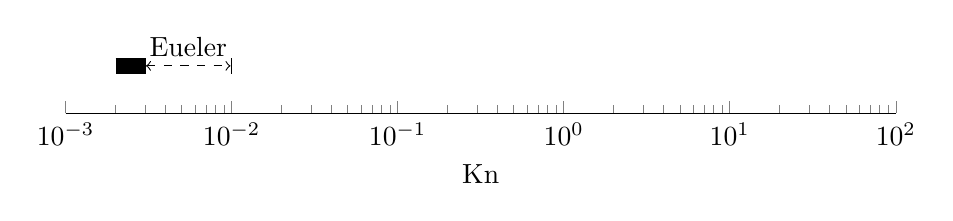
\begin{tikzpicture}
\begin{axis}[
    y=3cm,            % y unit vector
    hide y axis,        % hide the y axis
    xmode = log,        % logarithmic x axis
    axis x line*=bottom,% only show the bottom x axis line, without an arrow tip
    xmin=1e-3, xmax=1e2,% range for the x axis
    xlabel = Kn,
    width=\textwidth,
]
\addplot [no markers, line width=6pt] table {%
0.002 1
0.003 1
};
\draw [|<->|,dashed] (axis cs:0.003,1) -- (axis cs: 0.01,1) node[midway,above] {Eueler};
\end{axis}
%\begin{scope}[decoration=brace]
%	\draw [decorate] (current axis.south-|0.003) -- (current axis.south-|0.01) node[midway,above] {Eueler};
%\end{scope}
%\draw [] (axis cs:0.25,2.1) node[above] {\(T\)};
%\begin{scope}[decoration=brace]
%\pgfdecorationsegmentamplitude=5pt
%\draw[decorate] (T2.south east) -- (T0.south west) node[midway,below=\pgfdecorationsegmentamplitude] {Part 1};
%\draw[decorate] (T14.south east) -- (T3.south west) node[midway,below=\pgfdecorationsegmentamplitude] {Part 2};
%\draw[decorate] (T20.south east) -- (T15.south west) node[midway,below=\pgfdecorationsegmentamplitude] {Part 3};
%\end{scope}
\end{tikzpicture}